%% --------------------------------------------------------------------------
% LaTeX template for the XLIV CILAMCE
%
% This latex document tries to copy the Microsoft Word template.
% --------------------------------------------------------------------------
\documentclass[a4paper,10pt]{book}

% PACKAGES USED - packages that need to be previously installed on your computer
\usepackage[lmargin=2.5cm, rmargin=2.5cm, tmargin=2.5cm, bmargin=2.5cm ]{geometry}
\usepackage{graphicx}
\usepackage{times}
\usepackage{indentfirst}
\usepackage{fancyhdr}
\usepackage{titlesec}
\usepackage[english]{babel}
\usepackage{parskip} 
\usepackage{setspace}

% Mathematical Symbols
\newcommand{\dgds}{\boldsymbol{g_\sigma}}
\newcommand{\Dll}{\boldsymbol{D}}
\newcommand{\Dllmod}{\boldsymbol{D^{*}}}
\newcommand{\Dllepvp}{\boldsymbol{D}^{epvp}}
\newcommand{\dstrain}{\boldsymbol{\dot{\varepsilon}}}
\newcommand{\dstraine}{\boldsymbol{\dot{\varepsilon}}^{e}}
\newcommand{\dstrainp}{\boldsymbol{\dot{\varepsilon}}^{p}}
\newcommand{\dstrainv}{\boldsymbol{\dot{\varepsilon}}^{vp}}
\newcommand{\straineqp}{\bar \varepsilon^p}
\newcommand{\dstrainsh}{\boldsymbol{\dot{\varepsilon}}^{sh}}
\newcommand{\dstraincr}{\boldsymbol{\dot{\varepsilon}}^{cr}}
\newcommand{\dstress}{\boldsymbol{\dot{\sigma}}}

\newcommand{\ex}{\boldsymbol{e}_x}
\newcommand{\ey}{\boldsymbol{e}_y}
\newcommand{\ez}{\boldsymbol{e}_z}

\newcommand{\onell}{\boldsymbol{1}}
\newcommand{\strain}{\boldsymbol{\varepsilon}}
\newcommand{\straincr}{\boldsymbol{\varepsilon}^{cr}}
\newcommand{\straine}{\boldsymbol{\varepsilon}^{e}}
\newcommand{\strainp}{\boldsymbol{\varepsilon}^{p}}
\newcommand{\strainsh}{\boldsymbol{\varepsilon}^{sh}}
\newcommand{\strainshCEB}{\varepsilon_{sh}}
\newcommand{\strainvp}{\boldsymbol{\varepsilon}^{vp}}
\newcommand{\stress}{\boldsymbol{\sigma}}
\newcommand{\zerol}{\boldsymbol 0}

%%%%%%%%%%%%%%%%%%%%%%%%%%%%%%%%%%%%%%%%%%%%%%%%%%%%%%%%%%%%%%%%%
%%%%%%%%%%%%%%%%%%%%%%%%%%%%%%%%%%%%%%%%%%%%%%%%%%%%%%%%%%%%%%%%%
%%% My Additional Packages
%%%%%%%%%%%%%%%%%%%%%%%%%%%%%%%%%%%%%%%%%%%%%%%%%%%%%%%%%%%%%%%%%
\usepackage[utf8]{inputenc}
\usepackage{amssymb} %Mathematics
\usepackage{amsfonts}%Mathematics
\usepackage{amsmath,amscd}%Mathematics
\usepackage{amsthm}%Mathematics
\usepackage{mathrsfs}%Mathematics font
\usepackage{xspace}
\usepackage{booktabs}
\usepackage{stmaryrd}%Particular Brackets
\usepackage{graphicx} %Tables and Figures
\usepackage{subfigure}
\usepackage{url}
\usepackage{hyperref}
\usepackage{cleveref}
\usepackage{./pkg-crefNames}
\usepackage[labelsep=period]{caption}

%BibTeX compatible with the CILAMCE format
\usepackage[numbers,sort&compress]{natbib}

\setlength{\bibsep}{0pt plus 0.3ex}

\renewcommand*{\bibfont}{\small}

\makeatletter
\renewcommand\bibsection
{
  \section*{References}
}



\renewenvironment{thebibliography}[1]
      {\section*{\refname}%
       \@mkboth{\MakeUppercase\refname}{\MakeUppercase\refname}%
       \list{\@biblabel{\@arabic\c@enumiv}}%
            {\settowidth\labelwidth{\@biblabel{#1}}%
             \leftmargin\labelwidth
             \advance\leftmargin-10pt% change 20 pt according to your needs
             \advance\leftmargin\labelsep
             \setlength\itemindent{10pt}% change using the inverse of the length used before
             \@openbib@code
             \usecounter{enumiv}%
             \let\p@enumiv\@empty
             \renewcommand\theenumiv{\@arabic\c@enumiv}}%
       \sloppy
       \clubpenalty4000
       \@clubpenalty \clubpenalty
       \widowpenalty4000%
       \sfcode`\.\@m}
      {\def\@noitemerr
        {\@latex@warning{Empty `thebibliography' environment}}%
       \endlist}
\renewcommand\newblock{\hskip .11em\@plus.33em\@minus.07em}
\makeatother




\makeatother
\bibliographystyle{./bib-cilamce}
%\bibliographystyle{plain}


%%%%%%%%%%%%%%%%%%%%%%%%%%%%%%%%%%%%%%%%%%%%%%%%%%%%%%%%%%%%%%%%%
%%%%%%%%%%%%%%%%%%%%%%%%%%%%%%%%%%%%%%%%%%%%%%%%%%%%%%%%%%%%%%%%%

% CONFIGURATION
\renewcommand*\arraystretch{1.5}
\renewcommand*\thesection{\arabic{section}}
%\hyphenpenalty=10000 % You can uncomment this to avoid hyphenization
\titleformat*{\section}{\large\bfseries}
\titleformat*{\subsection}{\bfseries}
\titlespacing\section{0pt}{20pt plus 2pt minus 2pt}{12pt plus 2pt minus 2pt}
\titlespacing\subsection{0pt}{20pt plus 0pt minus 0pt}{12pt plus 0pt minus 0pt}
\setlength{\parskip}{0pt} % Spacing between paragraphs
\setlength{\parindent}{0.75cm} % Paragraph identation
\setlength\abovecaptionskip{6pt}

% --------------------------------------------------------------------------
% DO NOT EDIT - SPECIAL HEADINGS OF XLIII CILAMCE
% --------------------------------------------------------------------------
\fancypagestyle{first}
{
\fancyhf{}
\fancyfoot[RO]{\footnotesize \textit{CILAMCE-2024 \\
Proceedings of the XLV Ibero-Latin-American Congress on Computational Methods in Engineering, ABMEC\\
Maceió, Alagoas, November 11-14, 2024}}
\renewcommand{\headrulewidth}{.0pt}
\renewcommand{\footrulewidth}{.5pt}
}

\pagestyle{fancy}
\fancyhf{}

\fancyfoot[LE]{\footnotesize \textit{CILAMCE-2024\\
Proceedings of the XLV Ibero-Latin-American Congress on Computational Methods in Engineering, ABMEC\\
Maceió, Alagoas, November 11-14, 2024}}

\fancyfoot[RO]{\footnotesize \textit{CILAMCE-2024\\
Proceedings of the XLV Ibero-Latin-American Congress on Computational Methods in Engineering, ABMEC\\
Maceió, Alagoas, November 11-14, 2024}}




\renewcommand{\headrulewidth}{.5pt}
\renewcommand{\footrulewidth}{.5pt}

% --------------------------------------------------------------------------
% PLEASE, EDIT THIS!
\fancyhead[LE]{\footnotesize \textit{Finite Element Analysis of Rock Deformation in Deep Twin Tunnels}}
\fancyhead[RO]{\footnotesize \textit{Felipe P. M. Quevedo, Carlos A. M. M. Colombo, Bianca M. Girardi, Denise Bernaud, Samir Maghous}}
% --------------------------------------------------------------------------

\begin{document}\thispagestyle{first}

% --------------------------------------------------------------------------
% DO NOT EDIT - LOGO OF XLIII CILAMCE
% --------------------------------------------------------------------------

\begin{figure}[ht!]
\vspace{-30pt}
\flushright

\includegraphics[width=4.3cm]{Figures/logo.png}
%scale=0.25
\end{figure}

% --------------------------------------------------------------------------
% TITLE OF PAPER
% --------------------------------------------------------------------------

\noindent
\textbf{\Large
Finite Element Analysis of Rock Deformation in Deep Twin Tunnels} 
\vspace{18pt} % <- keep this vertical space!

% --------------------------------------------------------------------------
% AUTHORS
% --------------------------------------------------------------------------

\noindent Felipe P. M. Quevedo$^1$, Carlos A. M. M. Colombo$^1$, Bianca M. Girardi$^1$, Denise Bernaud$^1$, Samir Maghous$^1$

\vspace{18pt} % <- keep this vertical space!

\noindent $^1$\textit{Federal University of Rio Grande do Sul}

\noindent \textit{Av. Osvaldo Aranha, 99, Porto Alegre, 90.035-190, RS, Brazil}

\noindent \textit{motta.quevedo@ufrgs.br, ca-colombo@hotmail.com, eng.biancagirardi@gmail.com}

\noindent \textit{denise.bernaud@ufrgs.br, samir.maghous@ufrgs.br}


\vspace{18pt} % <- keep this vertical space!

% --------------------------------------------------------------------------
% ABSTRACT
% --------------------------------------------------------------------------

\noindent \textbf{Abstract.}
Relying upon a three-dimensional finite element analysis, this contribution investigates the instantaneous irreversivel response induced by the constitutive behavior of the rock mass in the convergence profile of twin tunnels. At the rock material level, elastoplastic state equations based on a Drucker-Prager yield surface with an associated flow rule are adopted in the modeling. As regards the tunnel support, the formulation accounts for the presence of an elastic shotcrete-like lining. From a computational point of view, the deactivation-activation method is used to simulate the excavation process and the installation of the lining. The accuracy of the finite element predictions is assessed through comparisons with the available analytical solutions formulated in a simplified scenario for the twin tunnel configuration. A parametric study investigates the mutual interaction induced by the proximity of the tunnels.

\vspace{18pt} % <- keep this vertical space!

\noindent \textbf{Keywords:} Twin tunnels, Elastoplasticity, Finite element modeling


% --------------------------------------------------------------------------
\section{Introduction}\label{sec:introduction}
% --------------------------------------------------------------------------
Many design methods often focus on single tunnels, but twin tunnels are a common occurrence. The interaction between tunnels can be significant, especially when the spacing between them is minimal. Additionally, many twin tunnels incorporate transverse galleries, introducing a localized effect on displacements and stresses. Also, the rheological behavior of the rock mass and lining plays a crucial role in how stress and displacements fields evolve over time. While the simulation of tunnel convergence in single tunnels has been widely investigated and reported in published
literature, few works have addressed the computational evaluation of deformation in twin tunnels. Some studies on deep twin tunnels can be found at \citet{Spyridis2015}, \citet{Chen2019}, \citet{MA2020}, \citet{Fortsakis2021}, \citet{chortis2021a}, \citet{chortis2021b}, \citet{GUO2021}, \citet{chortis2023a}, \citet{chortis2023b}. But less attention has been dedicated to assessing the mutual mechanical interaction induced by the excavation of the transverse gallery connecting the twin tunnels.


In this context, the main contributions of this paper can be summarized at both the material and tunnel analysis levels. At the material level, the constitutive state equations of the rock mass are developed using a coupled plasticity-viscoplasticity framework, which is suitable for clayey rocks. Both the immediate irreversible tunnel response (plasticity) and the delayed irreversible response (viscoplasticity) are captured using this approach. For the mechanical behavior of the concrete lining, the traditional linear elastic model are employed. At the structural analysis level, the deformation of the highly interactive components of the material system (i.e., rock mass and lining) resulting from the excavation of twin tunnels and transverse gallery is simulated using three-dimensional finite element simulations. The excavation and lining placement processes are simulated through the activation/deactivation technique. The constitutive models for the rock mass and lining and the associated numerical integration schemes, are implemented into the UPF/USERMAT customization tool [\citenum{ANSYS:2013b}] of the ANSYS standard software. This three-dimensional finite element analysis is specifically designed to address the interactions induced by the construction process, the proximity of twin tunnels, and the presence of the transverse gallery.

%Only full-length papers that have been orally presented will be published in the congress proceedings. It is extremely important that you prepare your full-length paper in strict accordance with the text formatting of this document, which can be enforced either using the pre-defined styles of this template file or manually setting the specifications described in the next section. After the preparation of your paper, you should generate a PDF file for submission. Only PDF files will be accepted by the online submission system.

% --------------------------------------------------------------------------
\section{Constitutive Model of the materials}\label{sec:format}
% --------------------------------------------------------------------------

The delayed behavior of constitutive materials is crucial in understanding the deformation of tunnel structures in deep clayey rocks (see for instance \citet{rousset1988}, \citet{Nguyen1987} or \citet{GIRAUD1996}). However, during the early stages of tunnel excavation, the rock mass around the tunnel undergoes severe loading and high strain rates, leading to significant instantaneous irreversible strains near the tunnel wall, which can impact the structure's long-term stability. The model formulation is based on earlier works by \citet{Nguyen1987} and \citet{rousset1988}. For brevity, only the main features of this model are summarized here, with detailed descriptions, applications, and validations available in \citet{quevedo2022b}. The finite element implementation of this model in the USERMAT procedure of ANSYS software is detailed in \citet{quevedo2022thesis}.

The elastoplastic-viscoplastic model for the rock mass is formulated based on a serial association of the elastoplastic and viscoplastic constitutive models. The local strain rate $\dstrain$ is split into three contributions $\dstrain = \dstraine + \dstrainp + \dstrainv$, so that the constitutive relationships relating the Cauchy stress rate $\dstress$ and strain rate components can be written as:
\begin{equation} \label{eq_constitutive_relationship_epvp}
	\dstress = \Dll : \dstraine = \Dll : (\dstrain - \dstrainp - \dstrainv).\;
\end{equation}



% The one-dimensional representation of the constitutive behavior is shown in Fig.~\ref{reological_scheme}.
%\begin{figure}[h!]
%	\centering
%	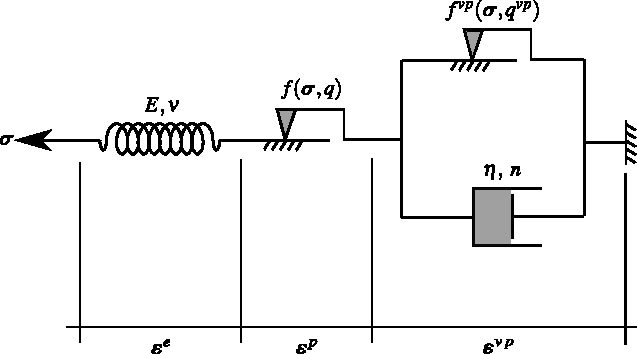
\includegraphics[scale=1]{Figures/Rheological representation.pdf}
%	\caption{Rheological representation of the elastoplastic-viscoplastic model.}
%	\label{reological_scheme}
%\end{figure}

In the above relationship, $\dstraine$, $\dstrainp$ and $\dstrainv$, represent respectively the elastic, plastic and viscoplastic strain rate, and $\Dll$ denote the fourth-order isotropic elastic linear constitutive tensor. Tensor $\Dll$ is defined by the rock mass elastic Young modulus $E$ and Poisson ratio $\nu$. The plastic strain rate is given by flow rule:
\begin{equation}
	\label{eq_plastic_flow}
	\dot \strainp = \left\{ 
	\begin{array}{ll} 
		\dot \lambda \dfrac{\partial g}{\partial \stress} &  \text{for } f > 0 \\ 
		\zerol, & \text{for } f \le 0 \\
	\end{array}\right.,
\end{equation}
where $\dot \lambda$ is the plasticity multiplier (obtained through the consistency condition  $\dot f = 0$) and $g$ is a potential flow function analogous to $f$ used to simulate the volume dilatation during the evolution of plastic deformations. However, for this analysis, was used associated plasticity, i.e., $g=f$. In this model is used a Drucker-Prager plastic flow surface given by
\begin{equation}
	\label{eq:f_Drucker_Prager}
	f(\stress,q) = f(I_1,J_2,q) = \beta_1 I_1 +\beta_2 \sqrt{J_2}-q(\alpha),
\end{equation}
which $I_1$ is the first invariant of the stress tensor, $J_2$ the second invariant of the deviator tensor and $\beta_1, \beta_2$ and $q(\alpha)$ are strength parameters related to the friction angle $\phi$ and cohesion $c(\alpha)$, respectively. In the present model Drucker-Prager surface been inner of the Mohr-Coulomb surface [\citenum{bernaud1991}], that is,
\begin{equation}
	\label{eq:f_DP_inscrita_MC}
	\beta_1 = \dfrac{(k-1)}{3}, ~~~ \beta_2 = \dfrac{(2k+1)}{\sqrt{3}}, ~~~
	q(\alpha) = 2\sqrt{k}~c(\alpha),
\end{equation}
where $k = (1+\sin{\phi})/(1-\sin{\phi})$. The internal variable $\alpha$ is the equivalent plastic strain $\straineqp$ used to simulate strain hardening/softening phenomena. However, for this study, we adopt perfect plasticity, meaning that c is a constant. For the viscoplasticity surface $f^{vp}$ the same surface is empolyed, but with $\phi^{vp}$ in $\beta_1$ and $\beta_2$, and $q^{vp} = 2\sqrt{k^{vp}}-c^{vp}$ where $k^{vp} = (1+\sin{\phi^{vp}})/(1-\sin{\phi^{vp}})$ and $c^{vp}$ is a constant, i.e., perfect viscoplasticity. 
 Numerical details of this implementation can be found in [\citenum{quevedo2022b}]. For viscoplastic flow rule we have,
\begin{equation}
	\label{eq_viscoplastic_flow}
	\dstrainv = \dot \lambda^{vp} \dfrac{\partial f^{vp}}{\partial \stress}
\end{equation}
In contrast to the plastic multiplier, the viscoplastic multiplier $\lambda^{vp}$ is independent of a consistency like condition. As a result, its expression is explicit. Based on the framework of generalized Perzyna's overstress theory [\citenum{perzyna1966}], its expression may be derived as follows:
\begin{equation} \label{eq_perzyna_model}
	\dot \lambda^{vp} = \dfrac{\Phi(\stress,q^{vp})}{\eta}~~~\text{and}~~~\Phi = \left\langle  \dfrac{f^{vp}(\stress,q^{vp})}{f_0} \right\rangle^n, \,
\end{equation} where $\Phi$ is the overstress function, $\eta$ is the dynamic viscosity constant, $n$ is the dimensionless parameter that gives the form of the power law, $f_0$ a parameter conveniently adopted and $\left\langle * \right\rangle$ is the McCauley function which is $0$ when $* <0$ , i.e. viscoplastic flow will only occur when the overstress function is positive.

In this coupled model, when $\phi=\phi^{vp}$, cohesion entirely controls the evolution of local mechanical fields. Specifically, when  $c \rightarrow \infty$ and $c^{vp} \rightarrow \infty$, the system achieves a purely elastic solution. The solution becomes purely elastoviscoplastic with $c \rightarrow \infty$, while a pure elastoplastic solution emerges with $c^{vp} \rightarrow \infty$. In the coupled analysis, condition $c^{vp} < c$ is adopted, allowing the viscoplastic domain to occur without plasticity. However, in the presence of plasticity, viscous effects become inevitable. Fig.~\ref{epvpdomains} illustrates these domains in principal stress space.
\begin{figure}[h!]
	\centering
	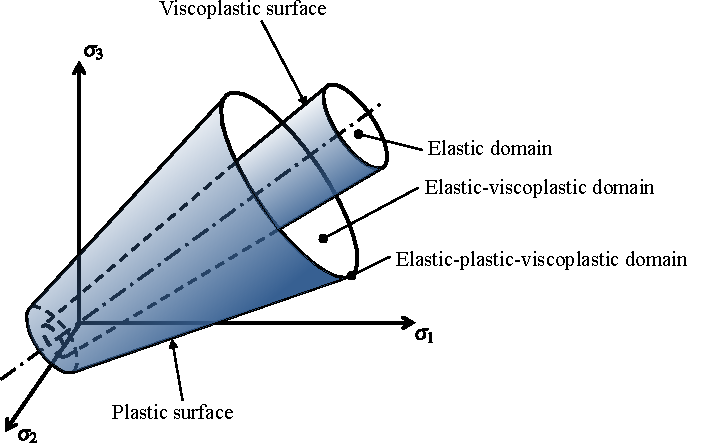
\includegraphics[scale=0.8]{Figures/Elastic-plastic-viscoplastic domains.pdf}
	\caption{Elastoplastic-viscoplastic domains.}
	\label{epvpdomains}
\end{figure}

A linear elastic constitutive model is used for the concrete lining, which can be expressed, within the framework of infinitesimal analysis, as:

\begin{equation} \label{eq:8}
	\dstress = \Dll : \dstraine;
\end{equation}
where, $\dstraine$ and $\Dll$ are respectively the elastic strain rate and the fourth-order isotrpoic elastic constitutive tensor dfined by the lining elastic Young modulus $E$ and Poisson ratio $\nu$.

% --------------------------------------------------------------------------
\section{Spatial and time discretization of the domain}\label{sec:format}
% --------------------------------------------------------------------------


% --------------------------------------------------------------------------
\section{Verification with unlined twin tunnel in elastoplastic medium}\label{sec:format}
% --------------------------------------------------------------------------


% --------------------------------------------------------------------------
\section{Numerical Results and Discussion}\label{sec:format}
% --------------------------------------------------------------------------

%Please follow these general instructions carefully: (a) type the body of the paper in 
%single column; (b)\textbf{ use no more than 7 pages (5 pages for papers at the Research Beginners 
%Mini-symposium)}, A4-sized, with 2.5 cm margins on all sides, and do not insert page numbers;
%(c) use 10pt Times New Roman throughout the body of the text, with 15pt for the paper's title
%13pt for first-level headings and 10pt for second-level headings; (d) always use either
%exactly 13pt-spaced lines (preferred) or single-spaced lines, with justified alignment; 
%(e) type no more than 200 words in the abstract; (f) cite references by last Name  [number],
%and list them consecutively in the reference list by the order of citation in the text 
%(the list should only include works that have been cited in the text); (g) provide good
%quality figures; (h) define all quantities, variables and symbols as soon as they first appear in the
%text; (i) use only SI units. We strongly encourage you to use the pre-defined styles of this template file, as they embed all text formatting described above. Full-length paper must be written in English. The general appearance of your paper should look like this document. 


% --------------------------------------------------------------------------
\subsection{Writing style} \label{subsec:writestyle}
% --------------------------------------------------------------------------

Please limit your paper by writing concisely, rather than by reducing figures or tables to a size at which symbols or labels would become difficult to read.

% --------------------------------------------------------------------------
\subsection{More detailed specifications} \label{subsec:additionalspecifications}
% --------------------------------------------------------------------------

The first page must include the paper's title (in sentence case), authors, affiliations, abstract, keywords, as well as the beginning of the text itself (i.e., the first section, which is usually the introduction). Do not insert a page break in between the keywords and the beginning of the text. Please follow strictly the line spacing defined next: either exactly 13pt-spaced lines (preferred) or single-spaced lines for the body of the text, with 20pt space before and 12pt space after first-level and second-level headings. If you use the pre-defined styles of this template, these specifications will be automatically applied.

\vspace{13pt}

\noindent \textbf{\textit{Remark 1: Author(s) and affiliation(s)}}. Type the authors’ names in regular (plain) type, flush left, including first name, middle initial(s) and last name. Group the authors by their affiliations with a superscript number. Each name or group of names must be followed by the corresponding affiliations and emails, which should be both in italics. A 12pt space must be left between the names and affiliations. If you use the pre-defined styles of this template, these specifications will be automatically applied.


\vspace{13pt}

\noindent \textbf{\textit{Remark 2: Abstract and keywords}}. Type ‘‘Abstract’’ in boldface, flush left, followed by a period. On the same line, type the abstract in regular (plain) format, justified alignment. The abstract should not exceed 200 words. Please pay attention to the line spacing between the authors affiliations and the abstract, as well as between the abstract and the keywords. If you use the pre-defined styles of this template, these specifications will be automatically applied. For the keywords, type ‘‘Keywords’’, followed by a colon, in boldface, flush left and type 3 to 5 keywords, separated by commas.

\vspace{13pt}

\noindent \textbf{\textit{Remark 3: Headings}}. First-level headings must be typed in sentence letters, 13 pt boldface type, flush left, as in Section 2 above. Use Arabic numbering (if you use the pre-defined styles of this template, automatic numbering is already built-in in the ‘‘1st Heading Cilamce-2024’’ style). Notice the line spacing before and after first-level headings. For second-level headings, use sentence letters, 10pt boldface type, flush left, with Arabic double numbering (if you use the pre-defined styles of this template, automatic double numbering is already defined). Notice the line spacing before and after second-level headings. Do not use third-level headings. Instead, use, at most, ''Remarks’’ (or the like), as shown here. These shall start with the word ‘‘Remark’’ (or the like) in boldface italics, followed by a number and a title (optional). The text that follows must be in regular (plain) format. Notice the line spacing before and after such paragraphs.

\vspace{13pt}

\noindent \textbf{\textit{Remark 4: Body of text}}. As said before, the body of the text should be typed in 10pt Times New Roman, using either exactly 13pt spaced lines (preferred) or single-spaced lines, with justified alignment. Start each paragraph with an indentation of 0.75 cm from the left margin, and allow no space between paragraphs. If you use the pre-defined styles of this template, these specifications will be automatically applied .

% --------------------------------------------------------------------------
\subsection{Equations, symbols and units}\label{subsec:equationsSymbolsUnits}
% --------------------------------------------------------------------------

Equations must be centered, right-numbered, with numbers enclosed in parentheses and placed flush right. Allow 6 pt line spacing before and after an equation. For example:

\vspace{6pt}
\begin{center}
\begin{equation}
q_r = -4pr^2k\frac{dT}{dr}.
\label{Eq1}
\end{equation}
\end{center}
\vspace{6pt}

Please pay attention to the punctuation after the equations, as equations are part of the text and must be punctuated accordingly.
When referring to an equation in the text, write \cref{Eq1}, except at the beginning of a sentence, wherein Equation (\ref{Eq1}) should be used. Please describe the notation adopted and be careful as to define all quantities, variables and symbols as soon as they first appear in the text. A nomenclature section is not necessary.

All data, including those shown in tables and figures, must be reported in SI units. Use decimal points rather than commas to indicate decimals.

% --------------------------------------------------------------------------
\subsection{Figures and tables}\label{subsec:figuresAndTables}
% --------------------------------------------------------------------------

Figures and tables should be inserted as close as possible to their first mentioning in the text. Embedded text and symbols must be clearly readable; avoid exceedingly small fonts. Supply good quality pictures and illustrations. Figures and tables and their captions should be centered in the text. Place figure captions below the figures and allow 12pt line spacing between both, and 20pt line spacing after the caption (i.e., before the subsequent text). Place table title above the table, leaving 20pt line spacing before the title and 6pt between the title and the table. Leave 20pt line spacing after the table (i.e., before the subsequent text). Examples are shown next:

\vspace{8pt}
\begin{table}[!ht]
\centering
\caption{Coefficients in constitutive relations}
\label{Table1}
\vspace{0pt}
\begin{tabular}{ccc}
\hline
Constitutive relation & Nomenclature & Value \\[-2pt] \hline
Turbulent tensor & C$_{\mu}$ & 0.09 \\[-3pt]
Turbulent tensor & C$_{\mu b}$ & 0.69 \\[-3pt]
Lateral lift & C$_{L}$ & 0.08 \\[-3pt]
Virtual mass & C$_{VM}$ & 0.8 \\[-3pt] \hline
\end{tabular}
\end{table}
\vspace{8pt}
Arabic numerals should be used in figures and tables (e.g., Figure \ref{Fig1}, Figure 2, Table \ref{Table1}, Table 2, etc). Refer to them in the text as Table \ref{Table1} and \cref{Fig1}, except at the beginning of a sentence, wherein Figure \ref{Fig1} should be used.

\begin{figure}[!ht]
\begin{center}
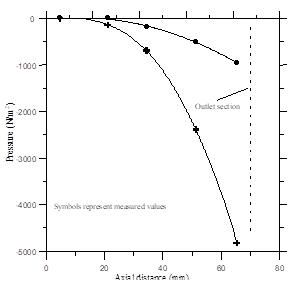
\includegraphics[scale=1.0]{Figures/Figure1.png}
\vspace{12pt}
\caption{Pressure variation along the nozzle: experimental data}
\label{Fig1}
\end{center}
\end{figure}
\vspace{8pt}

When constructing graphs or plots, do not forget to label coordinates and state the corresponding units. Similarly, label all columns/rows in tables and state corresponding units whenever applicable.

% --------------------------------------------------------------------------
\subsection{Permission}\label{subsec:permission}
% --------------------------------------------------------------------------

You are the sole responsible for making sure that you have the right to publish everything in your paper. If you use material from a copyrighted source, or from other authors, you may need to obtain permission from the copyright holder or the respective authors. An ``authorship statement'' must be placed at the end of your paper, immediately before the list of references, as shown further below. 

% --------------------------------------------------------------------------
\subsection{References}\label{subsec:references}
% --------------------------------------------------------------------------

References should be cited in the text by Last Name [number]. For example: ``In a recent work, \citet{Wriggers} proposed the method of  \citet{Bely}''. Numbers must be Arabic, enclosed in square brackets and used consecutively. References must be listed at the end of the paper, in a separate section entitled ``References''. They must be listed consecutively by the order of citation in the text. Type the word {``References''} in boldface, 13 pt Times New Roman type from the left margin, leaving 20 pt line spacing before and 12pt after. Then type the reference 9pt below it, in 9pt Times New Roman, with single-spaced lines (please do not leave blank spaces between references). See examples below. The list should only include works that are cited in the text.

% --------------------------------------------------------------------------
\section{Conclusions}\label{sec:conclusion}
% --------------------------------------------------------------------------

Type your conclusions or closing remarks here. Please be as concise and objective as possible. Do not make a summary of the paper, but instead list the main findings and results, even if these are only partial conclusions so far.

%-------------------------------------------------------------------------
\vspace{20pt}
\noindent \textbf{Acknowledgements.} This section should be positioned immediately after the Conclusion section. Type {Acknowledgements} in boldface, 10 pt Times New Roman type from left margin, leaving 20 pt line spacing before and 12pt after.
\vspace{12pt}

%--------------------------------------------------------------------------
\noindent \textbf{Authorship statement.} This section is mandatory and should be positioned immediately before the References section. The text should be exactly as follows:  The authors hereby confirm that they are the sole liable persons responsible for the authorship of this work, and that all material that has been herein included as part of the present paper is either the property (and authorship) of the authors, or has the permission of the owners to be included here. 

\bibliography{bibliography}

\end{document}
% --------------------------------------------------------------------------
